\section{SoDA -- Solid for Data Altruism}
\label{sec:soda}

This Section features an architecture designed to enable data altruism as a service, utilising the Solid protocol and ODRL policies to facilitate the sharing of personal data for altruistic purposes in a manner that respects data protection principles.
The policies are articulated using OAC and the DGAterms concepts related to data altruism.
Furthermore, we introduce the Solid Data Altruism application, SoDA, which allows (a) individuals to create policies for sharing their personal data for altruistic purposes, (b) data users to request access to datasets for altruistic purposes, and (c) data altruism organisations to manage metadata concerning available datasets.

\subsection{Solid architecture for data altruism}
\label{sec:architecture_soda}

The diagram presented in Figure~\ref{fig:soda_architecture} provides a broad summary of an architecture designed to implement data altruism as a service through the usage of the Solid protocol, with the central component being a Solid for Data Altruism application, known as SoDA.
The objective of this architecture is to start a proof of concept decentralised ecosystem for data altruism, emphasising the capability of data subjects to share personal data and data users to discover available datasets suitable for altruistic purposes, in line with data protection principles in the EU as the information disclosed about each dataset is limited to its data type and the intended purpose for its utilisation.

\begin{figure}[ht]
  \centering
  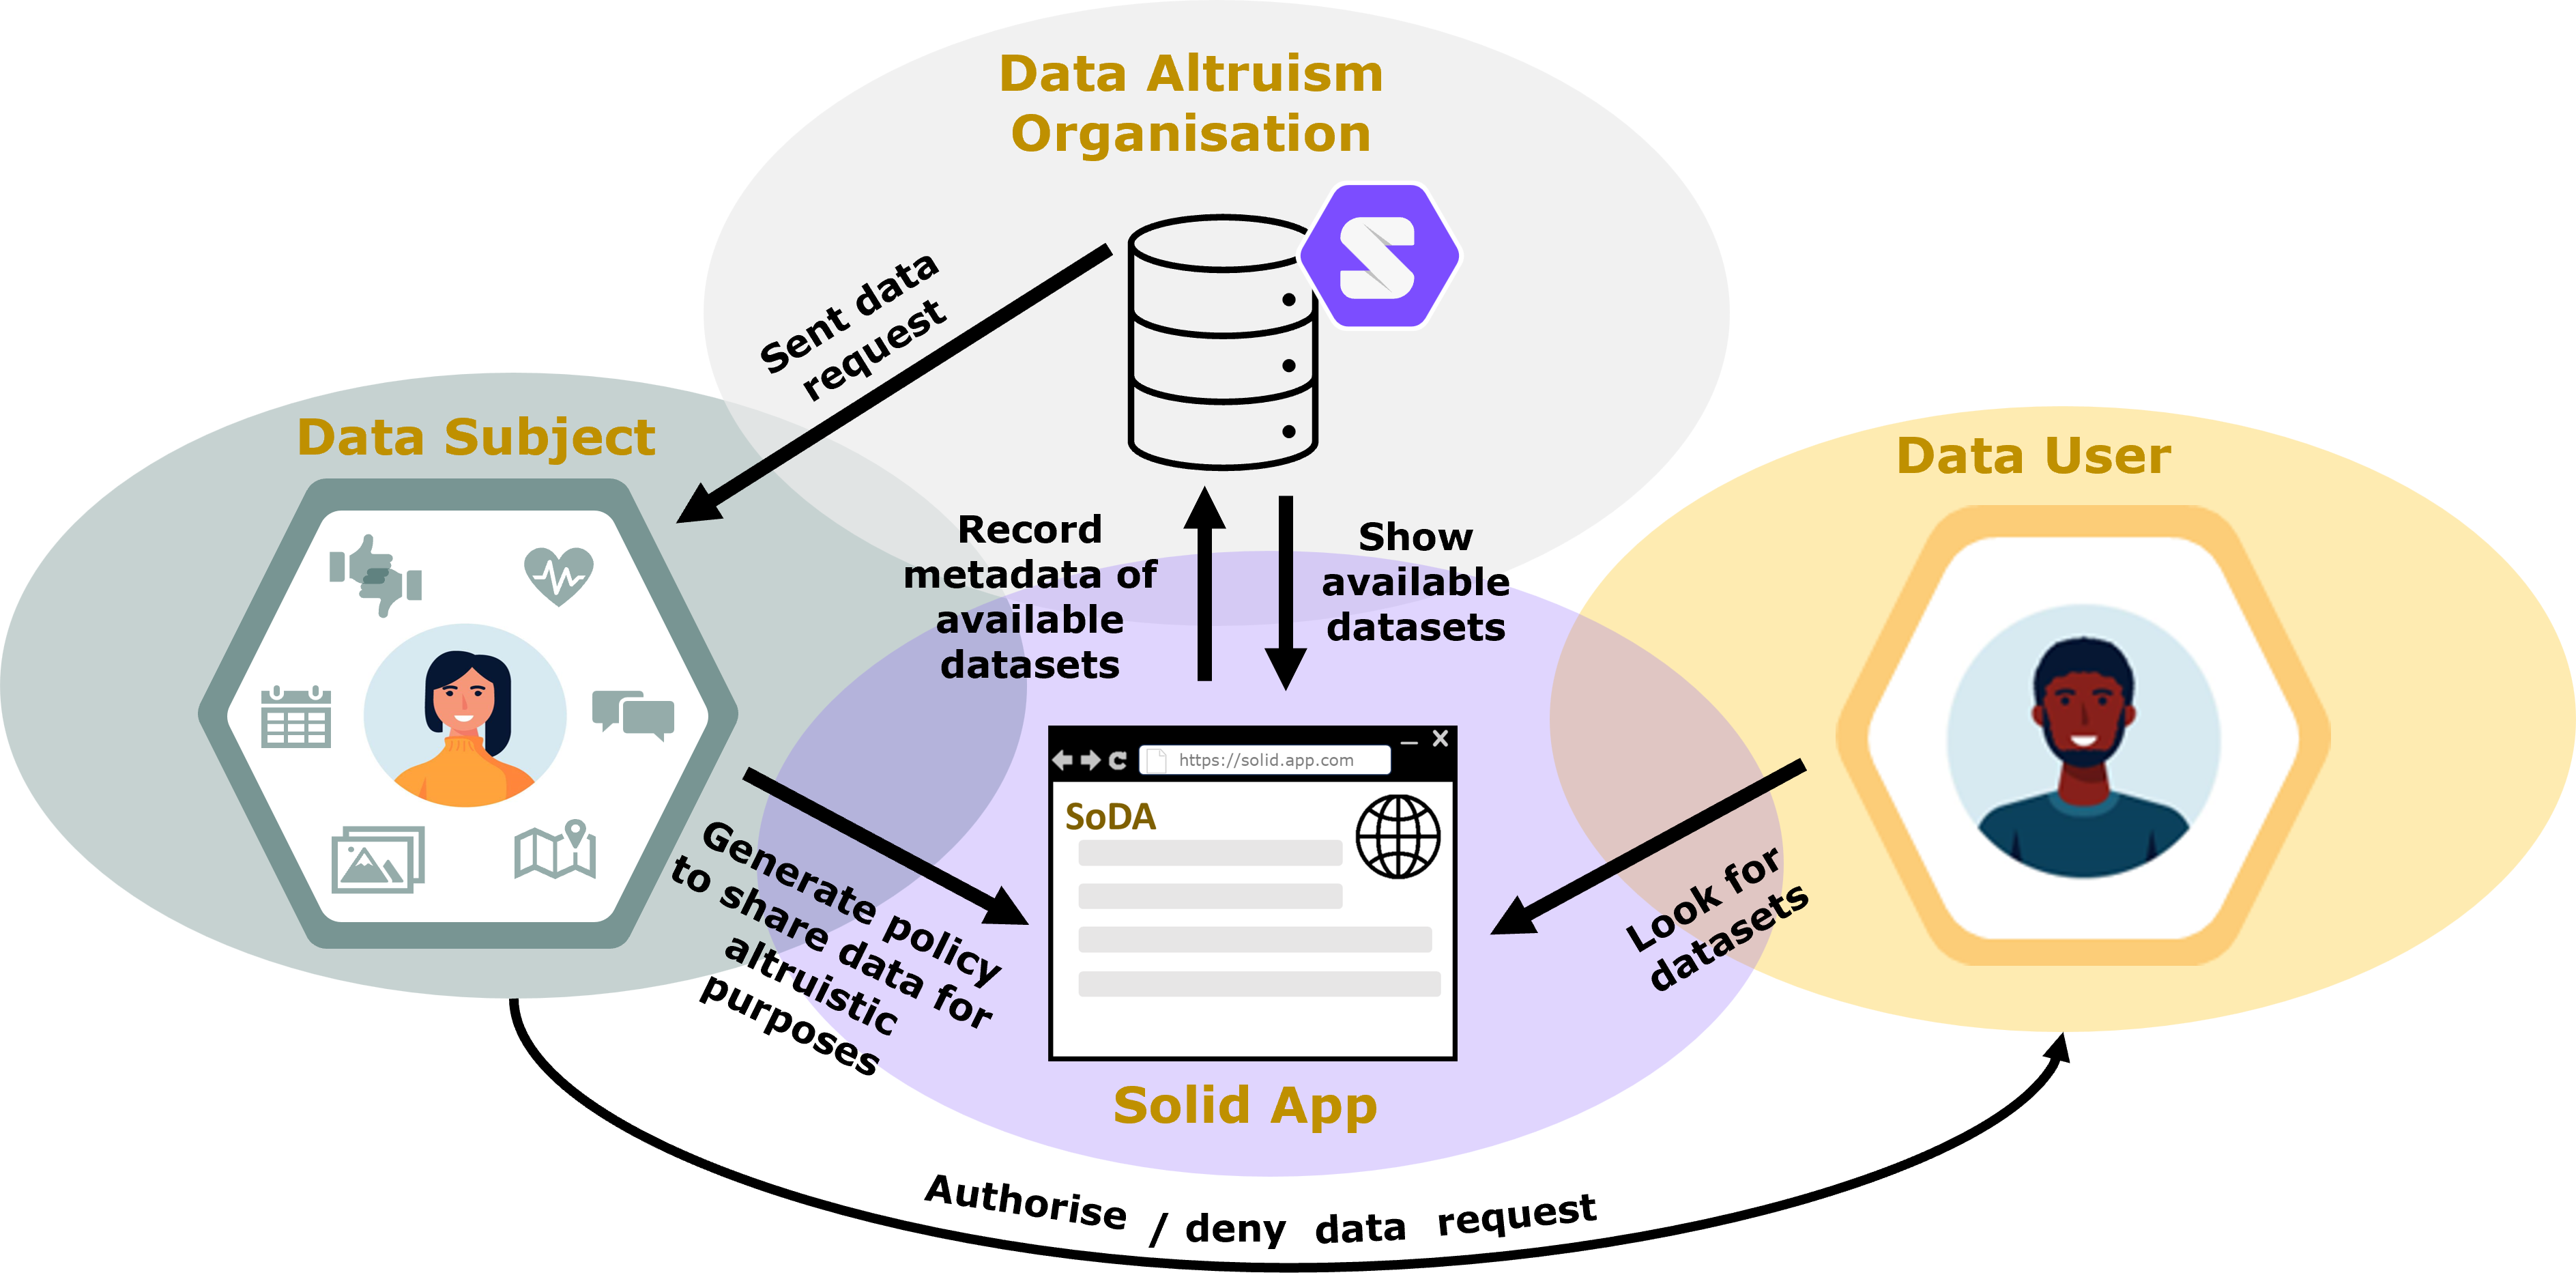
\includegraphics[width=\linewidth]{figures/chapter-7/architecture.png}
  \caption[SoDA architecture diagram.]{High-level diagram specifying an architecture to implement data altruism as a service using Solid and SoDA, a Solid application to edit policies/search for data for altruistic purposes, adapted from \cite{esteves_towards_2023}.}
  \label{fig:soda_architecture}
\end{figure}

As previously described, within a Solid-based architecture, users are recognised through a WebID and utilise Solid Pods to either store data or request access to stored data, adhering to the specifications outlined in the Solid protocol.
When personal data resides within Pods, GDPR and DGA requirements come into effect, with individuals who store their personal data in Pods being categorised as `data subjects'.
Additionally, both data subjects and data users administer data access via Solid applications.
In this setting, the SoDA application is introduced to:

\begin{enumerate}
    \item [(a)] empower data subjects to create policies for sharing their personal data with altruistic intent;
    \item [(b)] enable users to seek access to datasets based on their data type and intended purpose for usage; and
    \item [(c)] facilitate organisations in offering data altruism services by maintaining metadata about accessible datasets within their own Solid Pod, without the necessity of storing the data themselves, aligning with Solid's decentralised principles.
\end{enumerate}

With SoDA, individuals can craft data access policies governing their personal data, which are stored in their Solid Pod and can be shared with a data altruism organisation, which exclusively records metadata about the dataset and access conditions.
These records are leveraged to present available datasets to data users, safeguarding the privacy of data subjects by revealing solely the data type and permissible purpose of use, while concealing their identity. 
Should users identify datasets of interest, the data altruism organisation serves as an intermediary, forwarding data requests to the data subjects for them to authorise or deny access to the requested data.
Policies are modelled using OAC -- and by consequence, ODRL and DPV --, and DGAterms, and the catalogues of datasets kept by the altruistic company are based on DCAT.
Detailed instructions on how to install, launch, and use SoDA are available on the source code repository\footnote{\url{https://w3id.org/people/besteves/soda/repo}}.
Figures~\ref{fig:soda-ds} and~\ref{fig:soda-du} present a screenshot of SoDA's (i) policy editor UI and (ii) dataset request UI, respectively.

\begin{figure}[ht]
    \centering
    \fbox{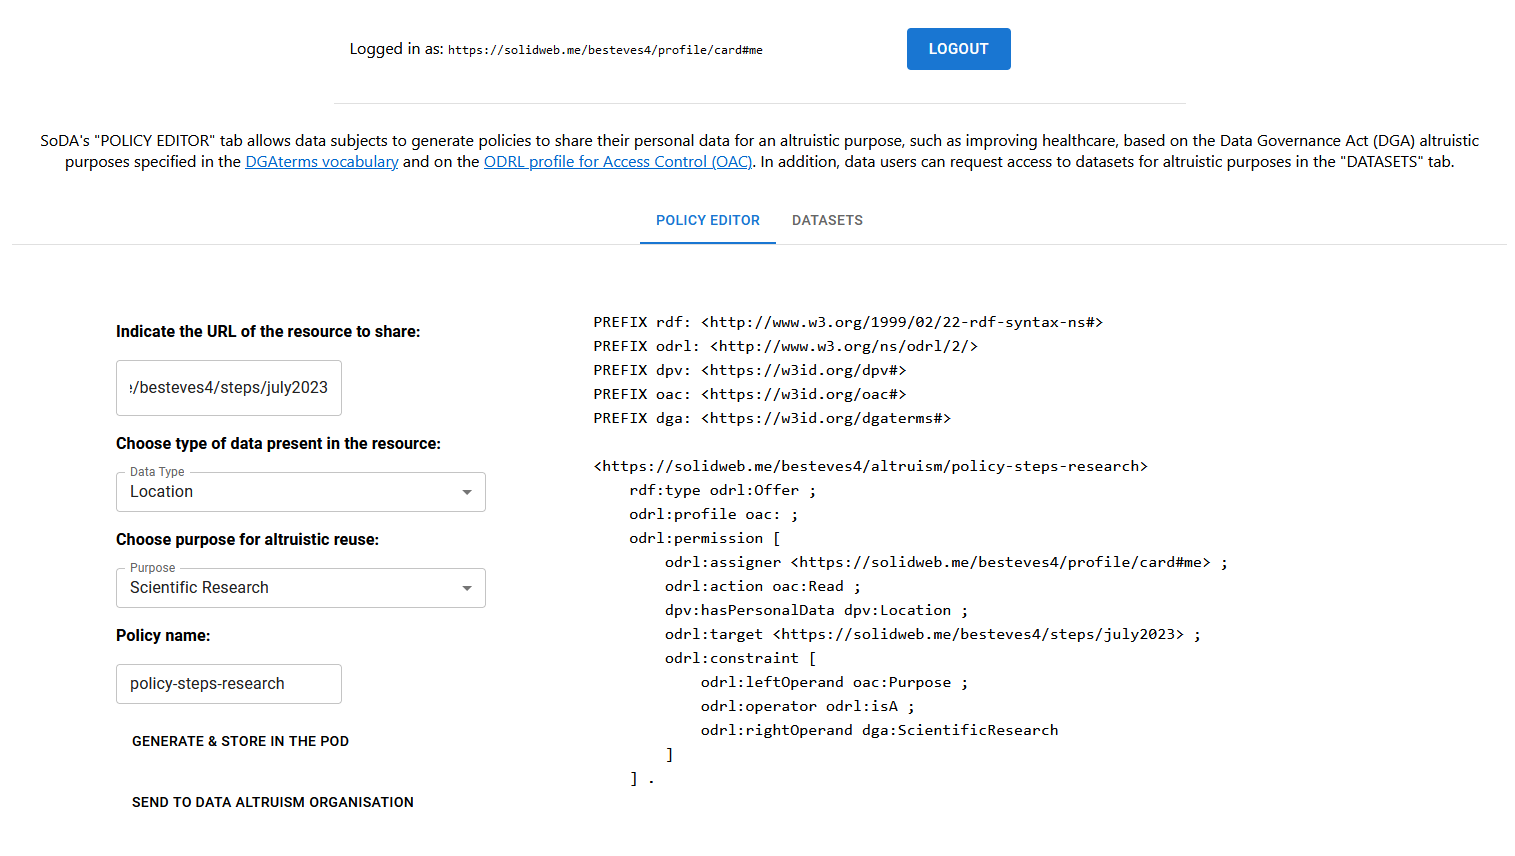
\includegraphics[width=\linewidth]{figures/chapter-7/policy-editor.png}}
    \caption[Screenshot of SoDA policy editor UI.]{Screenshot of SoDA policy editor UI, which generates OAC and DGAterms-based policies.}
    \label{fig:soda-ds}
\end{figure}

\begin{figure}[ht]
    \centering
    \fbox{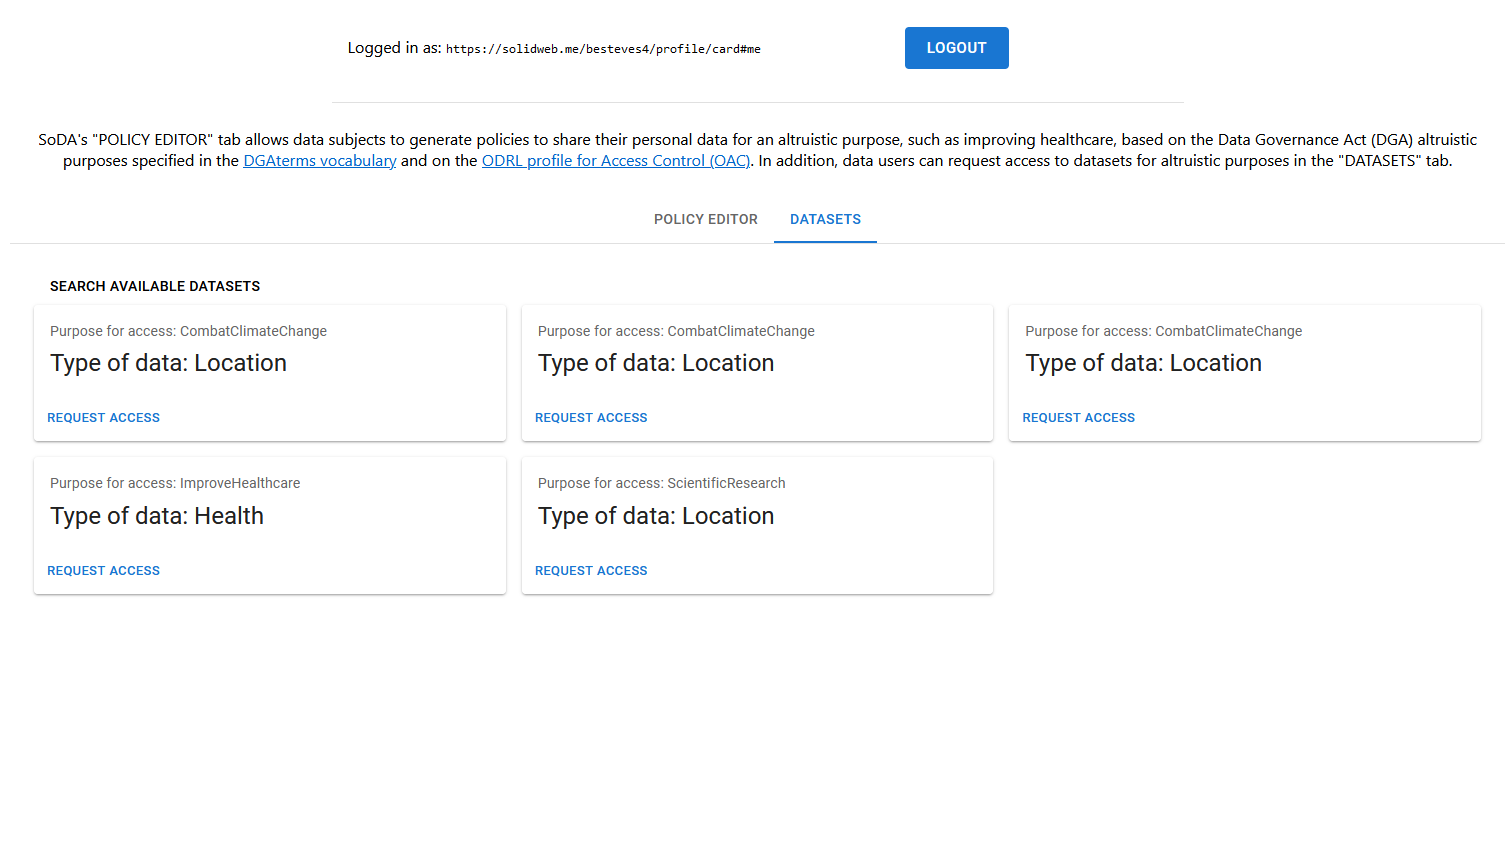
\includegraphics[width=\linewidth]{figures/chapter-7/datasets.png}}
    \caption[Screenshot of SoDA dataset request UI.]{Screenshot of SoDA dataset request UI, which allows data users to request access to a dataset for a specific purpose.}
    \label{fig:soda-du}
\end{figure}

\subsection{SoDA coverage, maintenance, and future work}
\label{sec:maintenance_soda}

SoDA is published and archived according to the methodology described in Section~\ref{sec:code_preservation}.
Furthermore, SoDA's source code is hosted at \url{https://w3id.org/people/besteves/soda/repo}, under the CC-BY-4.0 license.
Further information on this proof of concept application can be found at \url{https://w3id.org/people/besteves/demo/iswc23}, including a demonstration of the features of the app.
The repository can also be used by SoDA users to suggest new features to be added to the app and to report bugs through GitHub Issues.
Currently, SoDA's app coverage encloses terms from OAC/DPV taxonomies of purposes and personal data categories, focusing on the altruistic purposes described in the DGA.
As future work, SoDA can be extended to include all terms present in the previously mentioned DPV's data taxonomies, as well as to cover all constraints defined in the OAC profile, e.g., restrict legal bases, recipients or specify the technical and organisational measures used by data controllers to ensure the secure processing of personal data.
Additionally, user studies should be performed to assess the design choices included in the policy editor and dataset request UI, as well as to understand what type of additional controls people want to have on top of what is legally mandated, in particular, related to sharing data for altruistic purposes, e.g., temporal constraints or duties for the data user to fulfil after accessing the data.